\chapter{基于生成对抗网络的水下图像翻译}

\section{引言}

近年来,随着全球资源的日益短缺以及社会发展所产生的对资源的迫切需求,占据全球表面积71$\%$的海洋逐渐进入人们的视线。海洋中蕴含着丰富的资源,如果能够利用海洋资源,将缓解当下资源短缺的情况。目前,开发、研究和勘探海洋资源已成为国际社会关注的焦点。当研究水下环境时,清晰的水下图像和视频可以提供更有价值的信息,对于水下考古、水下勘探和水下开采等许多工作至关重要,然而原始的水下图像和视频通常受到水下环境中吸收、散射等影响,造成图像出现模糊、对比度低、雾状等效果,整体呈现蓝色调或绿色调,严重阻碍水下研究的进行。

提升水下图像的可视质量,解决雾化、模糊、色偏等问题的任务可视为水下图像清晰化,之前的传统工作可根据是否基于物理模型划分:基于非物理模型的方法是修改图像像素值以提高视觉质量,不需要考虑水下图像的成像原理和退质过程;基于物理模型的方法是从给定图像中估计成像模型的潜在参数。随着深度学习在低级视觉问题上取得的显著进展,数据驱动的方法越来越引起人们的关注,基于深度学习的方法根据其采用的主要模型可分为基于卷积神经网络的方法和基于生成对抗网络的方法。基于卷积神经网络的方法忠于原始的水下图像,基于生成对抗网络的方法旨在提高图像的感知质量,因基于生成对抗网络的方法更适于由多种因素导致的图像退化,因此本节设计的网络架构基于生成对抗网络。与第二章介绍的图像翻译相联系,水下图像清晰化也可看作一个图像翻译任务:给定一张水下退质图像,目的是生成一张高质量的去雾去噪、无色偏且高对比度的图像,本节利用第二章中介绍的分解表示实现非配对数据集情况下的水下图像清晰化。

\section{水的光学特性}

我们透过清澈的水观察水底的生物时,以为看到的场景与在空气中看到的一致,殊不知即使是这种清澈的水质,光在其中也存在严重的衰减,这一衰减主要是由吸收和散射引起的。水中的粒子吸收大部分光能量,导致颜色偏蓝绿色调,而散射过程包括光与水中颗粒(如沙子和浮游生物等)碰撞后的一系列方向变化,会对水下成像产生类似于雾天对室外视野的影响。

由于光衰减的波长相关性,水对光的吸收具有明显的选择性,图\ref{wavelength}显示出不同波长的光在水中的传播距离,红色光在4-5米后迅速消失,橙色光大多在5米深度处消失,黄色光在10米深度处完全消失,绿色光在20米深度处消失,且绿色波长在沿海水域传播得更远,蓝色则可以达到在水中传播50米深度以上才消失,在海洋中传播得更好。因此,水下图像颜色通常以偏蓝色或偏绿色为主(如图\ref{color}(a)所示),给水下中远距离的拍摄增加困难,一些有价值的信息会因吸收而丢失。

\begin{figure}[ht]
    \centering
	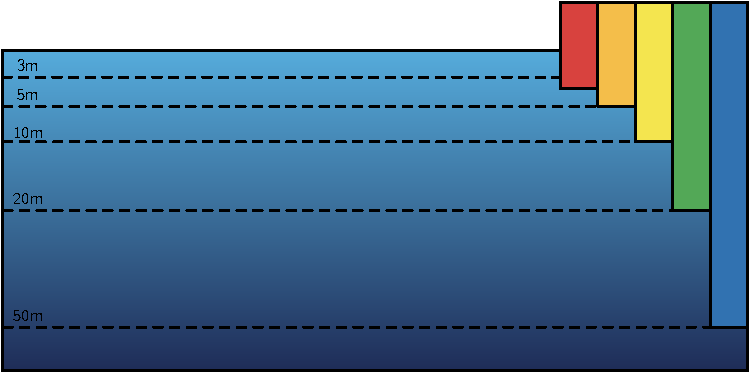
\includegraphics[width=\textwidth]{figs/wavelength.pdf}
	\caption{不同波长在水中的传播距离。图片来自文献\cite{han2018review}。}
	\label{wavelength}
\end{figure}

如果水对光仅存在吸收作用,那么可以通过增设人工光源来增加水下拍摄距离,但水对光还存在散射特性,随着人工光源的增强,散射作用愈见强烈。当我们用照相机拍摄水下场景时,根据Jaffe-McGlamery水下成像模型\cite{jaffe1990computer}\cite{mcglamery1980computer},由照相机拍摄的水下图像可以表示为以下分量的和:(1)直接分量$D$:场景中物体表面的反射光在传播过程中没有被散射的部分;(2)前向散射分量$F$:场景中物体表面的反射光在传播过程中发生小角度散射的部分;(3)后向散射分量$B$:介质中的粒子将入射到它们身上的光散射到许多其它方向,后向散射是这些光子到达照相机而形成的信号,不携带有关场景的信息。文献\cite{schechner2004clear}已经证明了$F\ll D$,前向散射对图像退化没有明显影响,所以仅考虑直接分量和后向散射分量,其中后向散射分量是导致水下图像质量下降的主要原因,会降低对比度,在水下图像中产生模糊和雾状效果(如图\ref{color}(b)所示)。

\begin{figure}[htp]
    \centering
	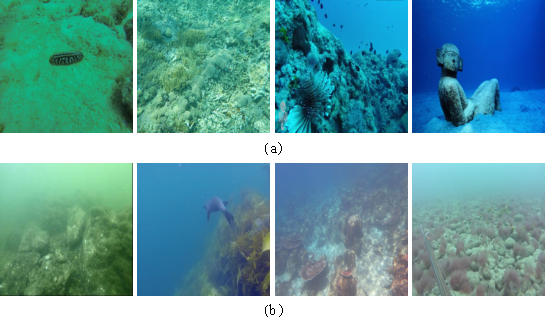
\includegraphics[width=\textwidth]{figs/color.pdf}
	\caption{(a)因水对光的选择吸收特性导致呈现蓝色调或绿色调的水下图像, (b)因水对光的散射特性而产生模糊和雾状效果的水下图像。图片来自文献\cite{fabbri2018enhancing}\cite{islam2019fast}。}
	\label{color}
\end{figure}

\section{模型算法}

现有两个域:水下图像域和清晰图像域,水下图像整体呈蓝绿色调且多显模糊,有雾状效果,而清晰图像可以看出图像中所有对象原本的颜色,对比度高且清晰度高。本节提出一个基于分解表示的框架,用于在无配对数据集情况下将水下图像域中的图像翻译到清晰图像域中。本节提出将图像分解到两个空间,具体来说,水下图像分解为:(1)色彩空间,其中含有吸收导致的水下图像特有的蓝绿色调;(2)信息空间,其包含了损失部分信息的内容和额外的雾、噪声等,清晰图像分解为:(1)色彩空间,其中包含对象和场景的真实色调;(2)信息空间,其中的信息丰富,拥有很多水下图像域没有的细节信息。

我们发现之前的基于分解表示的图像翻译方法虽然可以做到部分的颜色变化,但并不能保证水下图像中有用信息的完整性并添加来自清晰图像的信息(如图\ref{examples}),其翻译效果并不理想,为了解决这个问题,本节提出两个网络:特征提取网络和映射网络。特征提取网络在残差网络的基础上进行修改,旨在对映射到清晰图像域信息空间中的特征做进一步的特征提取和融合,尽可能多地学习清晰图像的信息。映射网络用于学习从水下图像域信息空间到清晰图像域信息空间的映射,在潜在空间中做映射是因为在紧凑的低维潜在空间中的映射原则上比在高维图像空间中更容易学习。通过我们提出的网络框架,可以在不同水下数据集上进行水下图像清晰化。

\begin{figure}[ht]
    \centering
	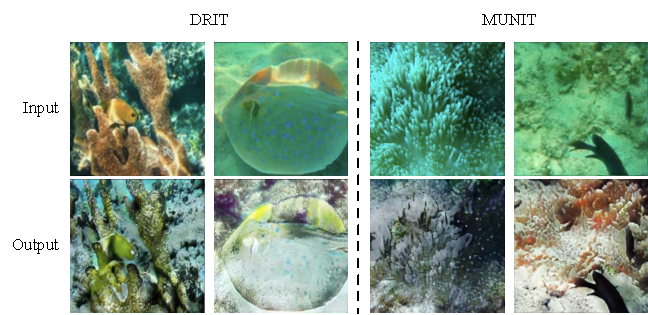
\includegraphics[width=\textwidth]{figs/DRIT_MUNIT_train_examples.pdf}
	\caption{DRIT和MUNIT在水下数据集上做图像翻译的效果。}
	\label{examples}
\end{figure}

\subsection{算法框架}

我们的目标是在无配对数据集的情况下,实现水下图像域$X$中的图像$x\in X$到清晰图像域$Y$中的图像$y\in Y$的翻译,如图\ref{architecture_underwater}所示,我们的框架包括色彩编码器$\{E_X^H, E_Y^H\}$,信息编码器$\{E_X^I, E_Y^I\}$,生成器$\{G_X, G_Y\}$,映射网络$M$和特征提取网络$FE$。在$X\rightarrow Y$方向上,图像$x$经过色彩编码器$E_X^H$得水下图像的色彩特征$h_x=E_X^H(x)$,同时$x$经信息编码器$E_X^I$得水下图像的信息特征$i_x=E_X^I(x)$,类似地,图像$y$经色彩编码器$E_Y^H$得清晰图像的色彩特征$h_y=E_Y^H(y)$,经信息编码器$E_Y^I$得清晰图像的信息特征$i_y=E_Y^I(y)$。如果按照DRIT和MUNIT的方式,那么将简单地把$i_x$和$h_y$输入到$G_B$中,以得到生成的清晰域图像$\hat{y}=G_B(i_x, h_y)$,由图\ref{examples}展示的DRIT和MUNIT翻译结果,我们推断水下图像的信息特征可能不足,不能与清晰图像的色彩信息一起生成清晰的图像,在生成清晰图像前,最好将水下图像的信息特征与清晰图像的信息空间对齐,且清晰图像的信息特征包含的信息越多越好。基于此推断,我们提出:(1)对清晰域的信息做进一步特征提取的特征提取网络$FE$,即$i_y^{fe}=FE(i_y)$,使其可以学习局部密集的信息特征,包含更多的细节信息;(2)将水下图像的信息特征$i_x$映射到清晰图像的信息空间中的映射网络$M$,即$i_x^m=M(i_x)$,使信息特征$i_x^m$与$Y$域的信息空间对齐,需要注意的是,此时应与经过特征提取的信息空间对齐。然后将$i_x^m$和$h_y$输入到生成器$G_Y$中,得到生成的清晰图像$\hat{y}=G_Y(i_x^m, h_y)$,综合上述,可以得到完整的由水下图像翻译到清晰图像的过程:
\begin{equation}
\begin{split}
\hat{y}=G_Y(i_x^m, h_y)=G_Y(M(i_x), h_y)=G_Y(M(E_X^I(x)), E_Y^H(y))
\end{split}
\label{eq:underwater_X2Y}
\end{equation}
由$X\to Y$可以类比出$Y\to X$方向上的翻译过程:
\begin{equation}
\begin{split}
\hat{x}=G_X(i_y^{fe}, h_x)=G_X(FE(i_y), h_x)=G_X(FE(E_Y^I(y)), E_X^H(x))
\end{split}
\label{eq:underwater_X2Y}
\end{equation}

\begin{figure}[ht]
    \centering
	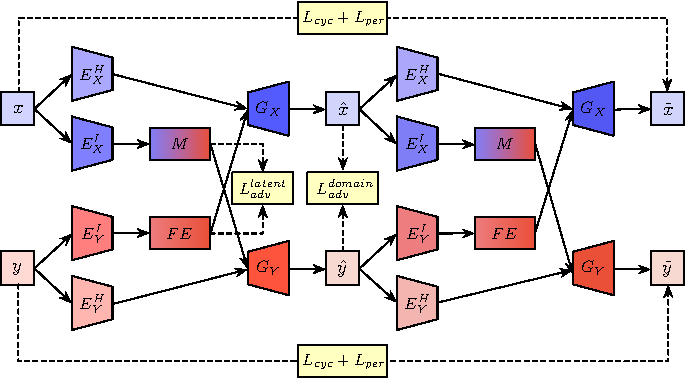
\includegraphics[width=\textwidth]{figs/architecture_underwater.pdf}
	\caption{水下图像清晰化模型示意图。}
	\label{architecture_underwater}
\end{figure}

\subsection{特征提取网络}

如图\ref{FE}所示,特征提取网络$FE$由9个特征提取网络块$FEB$组成,受ResNet\cite{he2016deep}和DenseNet\cite{huang2017densely}的启发,每个特征提取网络块$FEB$包括两组结构:一组包含卷积层$Conv$、实例归一化层$IN$\cite{ulyanov2016instance}和非线性激活函数$ReLU$\cite{nair2010rectified},一组包含卷积层$Conv$和实例归一化层$IN$,和ResNet不同的是,输入不仅与$FEB$的输出相加,还与第一组结构的输出按通道拼接,这样将残差块和密集连接整合到一起,既保留了残差块利用之前的特征的特点,又加入密集连接以渲染更多细节,从而达到对清晰图像的细节特征充分学习和整合的目的。经过9个$FEB$的顺序处理后,再将$FE$的输入与$FE$的输出相加,构成一个大的残差块,再次利用之前的特征。

\begin{figure}[ht]
    \centering
	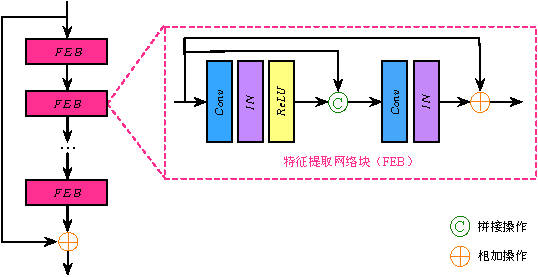
\includegraphics[width=\textwidth]{figs/FE.pdf}
	\caption{特征提取网络的网络结构示意图。}
	\label{FE}
\end{figure}

\subsection{映射网络}

映射网络将水下图像的信息特征映射到清晰图像的信息空间,需要做的是去掉水下图像中与雾、模糊等相关的信息,与清晰图像的信息空间对齐。针对去掉雾等信息,我们引入图像去雾相关操作,主要采用的是去雾文献\cite{hong2020distilling}提出的空间加权残差通道注意块$SWRCAB$,之前的去雾模块用全局平均池化操作来学习每个通道的权重,该权重将所有输入特征聚合并取平均,会忽略在不同通道上雾的浓度不同的问题,$SWRCAB$通过学习内容感知通道注意力以对严重退化的区域和信息通道施以更多关注,其首先用卷积层和非线性激活函数$Sigmoid$学习输入特征的空间权重,然后通过逐元素相乘的操作得到有空间权重的特征,最后通过一个全局池化层、全连接层和非线性激活函数$Sigmoid$来得到每个通道的注意力。类似于特征提取网络,由3个$SWRCABS$组成一个残差块,记作$RIR$,又用6个$RIR$构成最终的映射网络。

我们方法的关键之处在于使水下图像的信息特征可以映射到清晰图像的信息空间中,受之前的工作\cite{lee2018diverse}\cite{wan2020bringing}的影响,我们在此处用对抗损失来缩小两个域的信息空间之间的域差距,具体来说,我们训练一个潜在空间判别器$D^{L}$来判别$i_x^m$和$i_y^{fe}$,这个对抗损失可表示为:
\begin{equation}
\begin{split}
\mathcal{L}_{adv}^{latent} & = \mathbb{E}_x[\frac{1}{2}\log D^{L}(M(E_X^I(x))) + \frac{1}{2}\log(1-D^L(M(E_X^I(x))))] \\
& + \mathbb{E}_y[\frac{1}{2}\log D^{L}(FE(E_Y^I(y))) + \frac{1}{2}\log(1-D^L(FE(E_Y^I(y))))]
\end{split}
\label{eq:latent_GAN}
\end{equation}

\subsection{目标函数}

\subsubsection{循环一致性损失}

因为整个网络是在无配对图像的条件下训练的,所以借鉴CycleGAN\cite{zhu2017unpaired}的循环一致性损失来限制生成图像,以此弥补无配对数据集的缺陷。当给定$x\in X$和$y\in Y$,利用信息编码器和色彩编码器将其分别编码为$\{i_x, i_y\}$和$\{h_x, h_y\}$,再通过映射函数和特征提取函数分别将$i_x$和$i_y$编码为$i_x^m$和$i_y^{fe}$,通过交换两个域此时的信息特征和色彩特征,得到跨域生成图像$\{\hat{x}, \hat{y}\}$。为了实现循环,将$\{\hat{x}, \hat{y}\}$进行再分解,利用信息编码器和色彩编码器将$\{\hat{x}, \hat{y}\}$分别编码为$\{\hat{i}_x, \hat{i}_y\}$和$\{\hat{h}_x, \hat{h}_y\}$,然后$\hat{i}_x$经过映射函数得到$\hat{i}_x^m$,$\hat{i}_y$经特征提取函数得$\hat{i}_y^{fe}$,再次将两个域此时的信息特征和色彩特征进行交换,得到循环重建后的图像,即:
\begin{equation}
\begin{split}
\tilde{x}=G_X(\hat{i}_y^{fe}, \hat{h}_x) & =G_X(FE(\hat{i}_y), \hat{h}_x)=G_X(FE(E_Y^I(\hat{y})), E_X^H(\hat{x})) \\
\tilde{y}=G_Y(\hat{i}_x^{m}, \hat{h}_y) & =G_Y(M(\hat{i}_x), \hat{h}_y)=G_Y(M(E_X^I(\hat{x})), E_Y^H(\hat{y}))
\end{split}
\label{eq:cycle}
\end{equation}
经过两次跨域翻译后,生成的图像$\{\tilde{x}, \tilde{y}\}$应可以重建原始图像$\{x, y\}$(如图\ref{architecture_underwater}所示),为了对此进行约束,在此引入循环一致性损失:
\begin{equation}
\begin{split}
\mathcal{L}_{cyc}=\mathbb{E}_x[\parallel\tilde{x}-x\parallel_1] + \mathbb{E}_y[\parallel\tilde{y}-y\parallel_1]
\end{split}
\label{eq:cycle_consistenty}
\end{equation}

\subsubsection{感知损失}

感知损失利用预先训练好的VGG网络分别提取生成图像和真实图像的特征,并尽量使二者的特征相似,从而使生成图像和真实图像的高层信息相接近,避免计算像素级误差的损失无法捕捉感知区域的问题。在本节中,比较输入图像和循环重建图像之间的感知损失:
\begin{equation}
\begin{split}
\mathcal{L}_{per}=\mathbb{E}_{x,y}\sum_{i=1}^T\frac{1}{N_i}[\parallel\Phi_{VGG}^i(\tilde{x})-\Phi_{VGG}^i(x)\parallel_1 + \parallel\Phi_{VGG}^i(\tilde{y})-\Phi_{VGG}^i(y)\parallel_1]
\end{split}
\label{eq:perceptual}
\end{equation}
其中$T$代表总层数,$N_i$代表每一层元素的数量,$\Phi_{VGG}^i$代表VGG网络的第$i$层特征图。

\subsubsection{域对抗损失}

类似于DRIT\cite{lee2018diverse},我们引入域对抗判别器$\{D_X, D_Y\}$以判别每个域的真实图像与生成图像,在判别的过程中,$\{G_X, G_Y\}$致力于生成能够以假乱真的图像去欺骗域判别器,域对抗损失定义为:
\begin{equation}
\begin{split}
\mathcal{L}_{GAN}^{domain}& = \mathbb{E}_x[\log D_X(x)] + \mathbb{E}_x[\log(1-D_X(\hat{x}))] \\
& + \mathbb{E}_y[\log D_Y(y)] + \mathbb{E}_y[\log(1-D_Y(\hat{y}))]
\end{split}
\label{eq:GAN_loss}
\end{equation}

\subsubsection{KL损失}

我们在信息编码和色彩编码上应用KL散度来惩罚高斯先验和这些潜在分布的偏差,具体定义为:
\begin{equation}
\begin{split}
\mathcal{L}_{KL}& = \mathnormal{KL}(E_X^I(i_x|x)\parallel \mathcal{N}(0,1)) + \mathnormal{KL}(E_X^H(h_x|x)\parallel \mathcal{N}(0,1)) \\
 & + \mathnormal{KL}(E_Y^I(i_y|y)\parallel \mathcal{N}(0,1)) + \mathnormal{KL}(E_Y^H(h_y|y)\parallel \mathcal{N}(0,1)) \\
 & + \mathnormal{KL}(M(i_x^m|i_x)\parallel \mathcal{N}(0,1)) + \mathnormal{KL}(FE(i_y^{fe}|i_y)\parallel \mathcal{N}(0,1))
\end{split}
\label{eq:KL}
\end{equation}

\subsubsection{自重建损失}

为了保证分解得到的信息编码和色彩编码的完整性,类似于DRIT\cite{lee2018diverse},我们使由一幅图像分解得到的信息编码和色彩编码再经生成器,生成和原始输入尽量一致的图像,即$G_X(i_x, h_x)\approx x$,因此加入自重建损失,定义为:
\begin{equation}
\begin{split}
\mathcal{L}_{scyc}=\mathbb{E}_x[\parallel G_X(i_x, h_x)-x\parallel_1] + \mathbb{E}_y[\parallel G_Y(i_y, h_y)-y\parallel_1]
\end{split}
\label{eq:self_cyc}
\end{equation}

\subsubsection{总损失函数}

综合上述所描述的损失函数,得到最终的目标函数为:
\begin{equation}
\begin{split}
\min \limits_{G, E^I, E^H, M, FE} \max \limits_{D, D^L} \mathcal{L}_{total} 
& = \lambda_{adv}^{domain}\mathcal{L}_{adv}^{domain} + \lambda_{adv}^{latent}\mathcal{L}_{adv}^{latent}+ \lambda_{cyc}\mathcal{L}_{cyc} \\
& + \lambda_{per}\mathcal{L}_{per} + \lambda_{KL}\mathcal{L}_{KL} + \lambda_{scyc}\mathcal{L}_{scyc}
\end{split}
\label{eq:total}
\end{equation}
其中$\lambda_{adv}^{domain}$、$\lambda_{adv}^{latent}$、$\lambda_{cyc}$、$\lambda_{per}$、$\lambda_{KL}$和$\lambda_{scyc}$是超参数,用于控制和协调各项损失函数的权重以平衡损失。

\subsection{模型部署}

% 此处的引用看超哥的43页
\textbf{网络架构}~信息编码器和色彩编码器都由卷积神经网络构成,并加入$ReLU$激活函数\cite{nair2010rectified}和实例归一化\cite{ulyanov2016instance},采用实例归一化是因为水下图像数据集的场景多且杂,每个样本包含的独特信息都需要学习。生成器由残差块和转置卷积层构成,同样在每一层加入$ReLU$激活函数和实例归一化,除了最后一层用激活函数$Tanh$。判别器有两种,一种是简单的由堆叠卷积层构成的网络,用作对潜在空间进行判别,另一个采用多尺度判别器\cite{wang2018high},用于更好地学习整体轮廓和具体细节。

\textbf{训练细节}~整个网络基于PyTorch框架在256$\times$256分辨率的图像上训练,采用Adam\cite{kingma2014adam}优化算法并将批大小设为1,对于超参数,我们设置$\lambda_{adv}^{domain}=\lambda_{adv}^{latent}=1$,$\lambda_{cyc}=\lambda_{per}=\lambda_{scyc}=10$,$\lambda_{KL}=0.1$。

\section{实验}

\subsection{数据集设置}

$\mathbf{EUVP}$~由Islam等人\cite{islam2019fast}提出,包含大量感知质量高和感知质量低的配对和非配对水下图像,这些图像是在不同能见度、不同地点下进行的海洋探测和人机协同实验中收集的,除此之外,还包含一些从公开的YouTube视频中提取的图像,数据集中的图像包含不同的场景、水体类型和照明条件等,以适应广泛的自然变化。利用CycleGAN在由失真和未失真的水下图像构成的非配对数据集上训练,生成的失真图像和真实的未失真图像构成EUVP的配对数据集。配对数据集根据图像中的内容分为“Underwater Dark”(共5550对)、“Underwater ImageNet”(共3700对)和“Underwater Scenes”(共1364对),并提供一个可用于测试的“test samples”(共515对)。非配对数据集的获得则相对简单些,由6个志愿者根据其视觉感知效果的优劣分为两组,其中质量高的有3140张图像,质量低的有3195张图像。为了满足我们的训练需求,我们从非配对数据集中根据颜色、对比度和清晰度等图像属性进一步挑选,挑选的宗旨是:视觉感知效果好的域应仅包含清晰度和对比度高、没有色偏和雾状效果,同时包含尽量多的场景;视觉感知效果差的域应包含不同场景、不同浑浊度、不同颜色和不同照明条件的图像。最终,我们选出视觉效果优劣的图像分别为1310张和1295张用于训练(如图\ref{train}),分别用“test samples”中的配对图像和非配对图像中的“validation”做配对和非配对的测试。

\begin{figure}[ht]
    \centering
	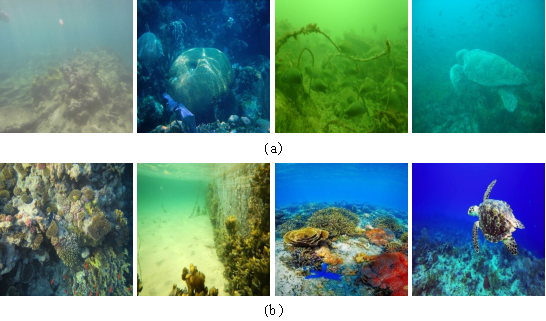
\includegraphics[width=\textwidth]{figs/train.pdf}
	\caption{(a)失真程度小、视觉效果好的水下图像, (b)失真程度大且视觉效果低的水下图像。图片来自文献\cite{islam2019fast}。}
	\label{train}
\end{figure}

$\mathbf{UIEB}$~由于缺乏充足且有效的训练数据,基于深度学习的水下图像增强方法的性能受到限制,由Li等人\cite{li2019underwater}提出的UIEB数据集提供了大量配对水下图像。Li等人从Google、YouTube和其它相关文献中收集图像,经过挑选,大多数图像被丢弃,剩下950张图像,对选出的图像分别用9种水下图像增强方法、2种图像去雾方法和1个水下图像增强的商业应用处理,每张图像都有对应的12张增强图像,找50个志愿者为每一个水下图像选择一个参考图像。若选择的参考图像中有超过半数的票被记为不满意,则其对应的原始水下图像视为具有挑战性的图像,并且将该图像的参考图像丢弃。由此共得到890对配对图像以及60张有挑战性的水下图像。之前的水下图像增强方法在评估的时候主要是使用合成的数据集或少数真实图像,UIEB数据集提供的参考图像数量大,颜色相对真实且可见性和亮度明显改善,在评估的时候更有说服力,因此将UIEB用作测试集。

$\mathbf{SUN}$~由Xiao等人\cite{xiao2016sun}提出的SUN数据集包含908个类别和131067张图像,本节仅关注此数据集中的水下图像,包含的场景有珊瑚礁、海洋深层、海洋浅层、水池和沉船,共713张图像,可用作测试集。

$\mathbf{RUIE}$~由Liu等人\cite{liu2019real}提出的RUIE数据集分为3个子集:水下图像质量子集(UIQS)、水下色偏子集(UCCS)和水下高级任务驱动子集(UHTS)。水下图像质量子集用UCIQE评价指标对这些图像打分,并按照所得分数排序,将其分为5类:A、B、C、D和E,每种水类型都有726张图像;水下色偏子集根据CIElab颜色空间中蓝色通道(红色-绿色偏差)的平均值生成,包含蓝色、蓝绿色和绿色三种颜色类型,每种类型都有100张图像;水下高级任务驱动子集包含集中海洋生物,目的是评估水下图像增强算法对高级计算机视觉任务(如分类和检测)的影响,为了探讨图像质量对检测精度的影响,将UHTS分为5个子集,每个子集包含60张图像。本节用UIQS测试不同算法在不同水条件下的性能,用UCCS评估不同算法校正色偏的能力。

\subsection{对比方法}

因本节将图像翻译应用到水下图像清晰化,所以不仅和图像翻译方法对比,也与几种水下图像增强方法对比。

\subsubsection{水下图像增强方法}

$\mathbf{UWCNN}$~Li等人\cite{li2020underwater}于2020年提出一种基于水下场景先验的水下图像增强卷积神经网络模型,称为UWCNN,此模型无需估计水下成像模型的参数,而是直接重建清晰的潜在水下图像。UWCNN的成功得益于其提出的水下合成数据集,因为基于深度学习的方法若缺乏充足有效的训练数据会限制模型的性能,因此Li等人在NYU-v2室内数据集\cite{silberman2012indoor}上根据水下成像物理模型和水下场景光学特性提出一个水下图像合成算法,可以模拟多种不同的水类型和降解水平。UWCNN可以在此数据集上训练以增强每种合成的水下场景类型,并推广到真实的水下图像中。

$\mathbf{UIE}$-$\mathbf{DAL}$~Uplavikar等人\cite{uplavikar2019all}认为水下图像因吸收和散射而呈现不同的水质,利用一个模型就可以对各种水质实现水下图像增强是极具挑战性的,UIE-DAL引入额外的妨害分类器消除不同水质对水下图像内容学习的干扰,从而很好地处理增强过程中水的多样性。模型在UWCNN合成水下数据集上训练,训练好的模型可泛化于真实水下图像。

$\mathbf{Deep~SESR}$~Islam等人\cite{islam2020simultaneous}提出的Deep SESR结合了密集残差子网,利用可解决特定水下颜色退化、图像清晰度不足和高级特征表示的多模态目标函数进行监督学习,辅以可指导网络学习全局对比度增强的前景区域(数据集提供),可同时处理水下图像增强和超分辨率的问题。因本节不进行超分辨性能的对比,所以仅利用其增强结果。

$\mathbf{Water}$-$\mathbf{Net}$~由fusion-based\cite{ancuti2012enhancing}得到启示,Li等人\cite{li2019underwater}采用多个预处理操作和融合策略,根据水下图像退化的特点,分别采用白平衡(WB)、直方图均衡化(HE)和Gamma校正(GC)算法处理原始水下图像以生成三个输入,将原始水下图像和处理后的三个输入图像输进提出的卷积神经网络Water-Net中,由公式\ref{eq:UIEB}可以看出最终得到的增强图像是三者融合,白平衡用于校正色偏,直方图均衡化和Gamma校正则用于提高对比度,提高黑暗区域的亮度。
\begin{equation}
\begin{split}
I_{en}=R_{WB}\odot C_{WB}+R_{HE}\odot C_{HE}+R_{GC}\odot C_{GC}
\end{split}
\label{eq:UIEB}
\end{equation}
其中$I_{en}$是增强结果,$\odot$代表矩阵的逐元素相乘,$R_{WB}$、$R_{HE}$和$R_{GC}$分别为原始水下图像经过WB、HE和GC处理后的结果,$C_{WB}$、$C_{HE}$和$C_{GC}$则为网络学到的置信图。

$\mathbf{UGAN}$~Islam等人\cite{fabbri2018enhancing}利用CycleGAN在挑选出的非配对失真和未失真水下图像上训练,将未失真图像和生成的失真图像配对,UGAN利用生成对抗网络在配对数据集上训练以增强水下图像。

\subsubsection{图像翻译方法}

$\mathbf{CycleGAN}$~Zhu等人\cite{zhu2017unpaired}提出的CycleGAN是非配对图像翻译的开山之作,在多个数据集上都有优异的表现,因此我们将其应用于水下图像转清晰图像的应用中。

$\mathbf{MSGAN}$~Mao等人\cite{mao2019mode}提出的MSGAN提出一个可以应用到多个框架的通用正则化项,在非配对图像翻译任务中,MSGAN以DRIT为基础框架,可以得到比DRIT更多样、更清晰的图像,因此我们在此不与DRIT对比,而是与效果更好的MSGAN对比。

$\mathbf{DSMAP}$~Chang等人\cite{chang2020domain}提出的DSMAP相比较MUNIT和DRIT做了进一步映射,我们提出的框架也是在DRIT和MUNIT的基础上进一步映射,虽都是再映射,但映射的方式不同,因此我们与DSMAP做对比以比较在水下图像清晰化任务上更有效的映射方式和网络框架。

\subsection{评价指标}

在生成水下图像时,不同的模型可能会产生不同的效果,存在不同程度的失真,进而导致视觉效果的降低。本节会提供在每个数据集上每个算法的视觉效果图,除此之外,为了在量化视觉图像质量,本节还会提供能够自动预测感知图像质量的定量指标。对水下图像质量的评估可根据是否需要参考图像分为有参考图像评价指标和无参考图像评价指标,常用的有参考图像评价指标有:SSIM\cite{wang2004image}、PSNR、MSE等,常用的无参考图像评价指标有UCIQE\cite{yang2015underwater}和UIQM\cite{panetta2015human}。

$\mathbf{MSE}$~均方误差(Mean Square Error)旨在提供代表两个信号之间相似性或失真的定量评分,通常情况下,一个信号是原始信号,另一个信号是从某种失真中恢复的,从数学上讲,两个信号之间的MSE可以表示为:
\begin{equation}
\begin{split}
MSE = \frac{1}{N}\sum_{i=1}^{N}(x_i - y_i)^2
\end{split}
\label{eq:example}
\end{equation}
其中$x$和$y$为两个信号,$x_i$和$y_i$是在位置$i$的像素,$N$是像素数量。MSE得分较低的结果表明其在图像内容方面更接近参考图像。

$\mathbf{PSNR}$~峰值信噪比(Peak Signal to Noise Ratio)在MSE的基础上再做一步处理,可用公式表示为:
\begin{equation}
\begin{split}
PSNR = 10\log_{10}\frac{L^2}{MSE}
\end{split}
\label{eq:example}
\end{equation}
其中$L$代表图像像素强度的动态范围(图像为255),PSNR得分较高的结果表明其在图像内容方面更接近参考图像。

$\mathbf{SSIM}$~结构相似性(Structural SIMilarity)由Wang等人\cite{wang2004image}提出,相比较MSE和PSNR侧重于内容的完整性与相似性,SSIM主要计算生成图像与真实图像之间的结构相似性。每幅图像都有其自己特定的结构,表现为图像的像素之间存在相关性,SSIM从此角度出发,比较生成图像与参考图像之间的亮度、对比度和局部结构。考虑从两个相比较图像的相同位置获取的局部区域块$x$和$y$,可将亮度$l(x,y)$、对比度$c(x,y)$和局部结构$s(x,y)$相乘得SSIM分数:
\begin{equation}
\begin{split}
SSIM=l(x,y)\cdot c(x,y)\cdot s(x,y) =(\frac{2\mu_x\mu_y + C_1}{\mu_x^2+\mu_y^2+C_1})(\frac{2\sigma_x\sigma_y+C_2}{\sigma_x^2+\sigma_y^2+C_2})(\frac{\sigma_{xy}+C_3}{\sigma_x+\sigma_y+C_3})
\end{split}
\label{eq:example}
\end{equation}
其中$\mu_x$和$\mu_y$分别为局部区域块$x$和$y$的均值,$\sigma_x$和$\sigma_y$则分别为局部区域块$x$和$y$的标准差,$\sigma_{xy}$代表去掉均值后局部区域块的互相关,$C_1$、$C_2$和$C_3$存在的意义在于保证被除数不为0。SSIM分数较高的结果表明其在图像结构和纹理方面与参考图像更接近。

$\mathbf{UCIQE}$~由于水对光的吸收和散射特性使水下图像呈现模糊、色偏、对比度下降等降质问题,使得评价空气中图像的指标(如FID)不适用于水下图像。根据CIELab颜色空间中的色彩统计,研究者发现清晰度和色彩因子可以很好地反映水下图像质量,且与人眼观看评价接近,在此基础上,水下彩色图像质量评估\cite{yang2015underwater}(Underwater Color Image Quality Evaluation)线性组合色度、饱和度和对比度,可表示为:
\begin{equation}
\begin{split}
UCIQE=C_1\times\sigma_c+C_2\times con_l+C_3\times\mu_s
\end{split}
\label{eq:example}
\end{equation}
其中$\sigma_c$、$con_l$和$\mu_s$分别为色度的标准差、亮度的对比度和饱和度的均值。UCIQE分数越高,说明结果在色度、饱和度和对比度之间有更好的平衡。

$\mathbf{UIQM}$~对于水下图像,不同波长的光吸收率不同会导致色偏,散射则会导致水下图像呈现模糊、噪声和雾状等效果,因此在评价水下图像质量时,水下图像质量评价\cite{panetta2015human}(Underwater Image Quality Measure)利用与感知水下图像质量有很好相关性的HSV模型,选择了主要由水介质特性而退化的色度、清晰度和对比度作为评价水下图像质量的属性,定义为:
\begin{equation}
\begin{split}
UIQM=c_1\times UICM+c_2\times UISM+c_3\times UIConM
\end{split}
\label{eq:example}
\end{equation}
其中UICM为图像色度度量,UISM为清晰度度量,UIConM为对比度度量,$c_1$、$c_2$和$c_3$是三者的权重系数,本文对其的设置分别为0.0282、0.2953和3.5753。UIQM的分数越大,说明结果与人类视觉感知越一致。

\subsection{实验结果与分析}

\begin{figure}
    \centering
	\includegraphics[width=\textwidth]{figs/EUVP_paired.pdf}
	\caption{对比方法和我们的方法在EUVP配对数据集上的测试结果。}
	\label{fig:euvp_paired}
\end{figure}

\begin{figure}
    \centering
	\includegraphics[width=\textwidth]{figs/EUVP_unpaired.pdf}
	\caption{对比方法和我们的方法在EUVP非配对数据集上的测试结果。}
	\label{fig:euvp_unpaired}
\end{figure}

\begin{figure}
    \centering
	\includegraphics[width=\textwidth]{figs/UIEB.pdf}
	\caption{对比方法和我们的方法在UIEB数据集上的测试结果。}
	\label{fig:UIEB}
\end{figure}

\begin{figure}
    \centering
	\includegraphics[width=\textwidth]{figs/SUN.pdf}
	\caption{对比方法和我们的方法在SUN数据集上的测试结果。}
	\label{fig:SUN}
\end{figure}

\subsubsection{主观定性评价}

我们在4个数据集上进行测试和评价,所用到的对比方法的代码均下载自作者公开的Github链接,其中水下图像增强或复原方法中部分方法有公开的预训练模型,我们均采用其预训练模型测试和评价,剩下未公开预训练模型的方法,我们按照其在论文中提到的方式训练,对于图像翻译方法,都采用和我们的方法相同的数据集训练。需要特别提到的是,UWCNN方法公开了针对8种水质的预训练模型,我们用每个预训练模型在UIEB数据集上测试并评价,发现typeI模型的效果最好,这也与UWCNN论文中展示的结果相符,因此后续图和表中展示的均为typeI预训练模型的结果。

EUVP数据集分为配对和非配对两部分,我们首先在配对数据集上测试,测试结果如图\ref{fig:euvp_paired}所示,可以看出我们的方法在细节学习和颜色校正上有很大优势。UWCNN、Water$-$Net和UGAN虽然也可以做到清晰化,但清晰化的作用有限,虽修正了部分颜色,使蓝色调和绿色调程度减轻,但整体仍呈现雾状的效果。视觉效果最差的为UIE$-$DAL和DSMAP,UIE$-$DAL整体色调变深变黑,细节损失严重,且不能生成背景为海水的部分。DSMAP细节损失更严重,只能看到大概的内容,造成这种结果可能是因为它原本用于风格迁移任务,所设计的网络不适合水下图像清晰化任务,且生成图像受所指引图影响严重,不能很好的恢复出水下图像原本的颜色。CycleGAN生成的图像整体看着清晰,但细节部分处理得不好,很容易出现网格纹路,第五张图像中的网格尤其明显。MSGAN也存在生成图像有网格的现象,除此之外,还倾向于生成黑色的色块,这种黑色色块的出现会大大降低视觉效果,使生成图像不逼真。Deep SESR和我们的方法在视觉上相差不大,都能兼顾细节和色彩的生成,但我们的方法在细节处更清晰,对颜色的校正能力更强。

我们在EUVP非配对数据集中挑选的水下图像以有浓雾为主,如图\ref{fig:euvp_unpaired}所示,对于有浓雾区域的图像,我们的方法可以在去雾校正颜色的同时保证背景的完整和清晰,从第二列和第三列的图像可以看出,只有我们的方法可以将其整体色调校正为白色,保留细节和边缘且保证生成图像色彩的斑斓。在此数据集上,UWCNN对去雾的作用最小,几乎是仅将图像的颜色做了变化,雾气没有做处理,UIE$-$DAL将图像的颜色都变暗且很多细节信息都有损失,它们的效果差可能是因为其是在室内数据集生成的水下图像上训练的,在真实水下场景的泛化能力有限。Water$-$Net和UGAN可以做到校正颜色,但整体效果偏朦胧。CycleGAN生成的图像可以去掉部分雾,但仍存在网格等纹路,使图像的视觉效果下降。综合来看,我们的效果最能达到清晰化目的。

UIEB数据集包含不同颜色、不同场景的水下图像,我们在此特意挑选了色调不同、场景不同、光照不同的几幅图像,图\ref{fig:UIEB}展示了我们的方法在绿色调和蓝色调的图像上都可以实现清晰化,并尽力将图像的颜色恢复至白色的色调,第一列图像尤其能体现我们的方法在颜色校正方面的性能,第三列和第五列的输入图像都呈现暗光照,我们的方法也可以将其去雾并点亮整幅图像。在颜色校正方面,UWCNN和Deep SESR表现最差,蓝绿色调去掉的程度有限,UIE$-$DAL虽可以去掉蓝绿色调,但其整体呈暗色调,物体本身的颜色也有部分丢失。MSGAN和DSMAP细节内容缺失得最多,边缘弱化,且生成很多杂纹。UGAN整体视觉效果一般,其问题仍为清晰度不够。Water$-$Net的训练集即UIEB数据集,并在相同的数据集上测试,因此它的效果是最接近参考图像的。

图\ref{fig:SUN}展示了在SUN数据集上的测试结果,相比较前三个数据集,在此增加展示游泳场场景的水下图像,综合来看,可以明显观察到我们的结果校正颜色的能力最好,尤其是第三列,我们的生成图像可有效去除水的光学特性的影响,第五列图像也能看出我们方法的优势,人和物体的生成都很逼真,且整体的色调与正常的空气中的图像一致。UWCNN在此数据集上的效果仍一般,颜色校正能力依旧低,UIE$-$DAL不仅没有校正颜色,还在输入图像的基础上加深了颜色,人物等具体内容很难看清。Deep SESR、Water$-$Net和CycleGAN有一定的校正颜色能力,Deep SESR在光照不强烈的水下图像上表现一般,无法使整体图像变亮,不过其有较好的清晰度,UGAN和MSGAN有一定的颜色的校正能力,但它们都存在边缘模糊的问题,导致清晰度不够。 

\subsubsection{客观定量评价}

上一小节展示了几种方法在4个数据集上的视觉效果,本小节将从客观角度描述在4个数据集上的测试结果。针对EUVP配对数据集和UIEB数据集这类有参考图像的数据集,我们用到的评价指标有MSE、PSNR、SSIM、UCIQE和UIQM,针对EUVP非配对数据集和SUN数据集,因其没有参考图像,因此只能用UCIQE和UIQM评价指标,UISM、UICM和UIConM是构成UIQM分数的组成部分,在分析结果的时候可以进行辅助,因此也在表中列出,但主要参考UCIQE和UIQM。在此注明:表中$\uparrow$代表此评价指标的值越大越好,反之$\downarrow$代表值越小越好;表中加粗的数字为最好的结果。

表\ref{tab:euvp_paired}是在EUVP配对数据集上的定量结果,在MSE、PSNR和SSIM评价指标上,我们的结果稍逊于Deep SESR,结合图\ref{fig:euvp_paired}可以发现,我们的视觉效果实际上优于Deep SESR,但在这三个指标上的结果不如Deep SESR的原因可能是我们的方法生成的图像可以更彻底地校正颜色,如图中的第二列和最后一列,而参考图像仍带有绿色,这是因为EUVP数据集中的参考图像是真实的水下图像,只是视觉效果相对较好,实际仍带有部分水下图像的特点,Deep SESR比我们的方法更接近参考图像,因此MSE、PSNR和SSIM的分数更高。UCIQE和UIQM评价指标是我们的方法最高,说明我们的方法有更好的平衡色度和清晰度的能力。DSMAP的结果毫无疑问是最差的,这与图\ref{fig:euvp_paired}的结果可对应,但意外的是,DSMAP的UIQM值却比水下图像增强方法高,可能是因为生成图像整体以黄色和黑色为主,有较强的对比度,而对比度的权重为3.5753,在UIQM的分数构成中占很大比重,因此其UIQM分数高。

\begin{table*}[ht]%\footnotesize
\centering
\caption{对比方法和我们的方法在配对EUVP数据集上的定量结果。}
  \begin{tabular}{c|ccc|ccccc}
    \hline\noalign{\smallskip}
    方法 & MSE$\downarrow$ & PSNR$\uparrow$ & SSIM$\uparrow$ & UCIQE$\uparrow$ & UIQM$\uparrow$ \\
    \noalign{\smallskip}\hline\noalign{\smallskip}
    UWCNN\cite{li2020underwater} & 478.8926 & 22.5549 & 0.8285 & 0.5341$\pm$0.0374 & 4.8583$\pm$0.4255 \\
    UIE-DAL\cite{uplavikar2019all} & 1816.8252 & 16.7337 & 0.7078 & 0.5521$\pm$0.0354 & 5.1255$\pm$0.2433 \\
    Water$-$Net\cite{li2019underwater} & 375.2734 & 24.0613 & 0.8451 & 0.5836$\pm$0.0380 & 5.0404$\pm$0.5389 \\
    Deep SESR\cite{islam2020simultaneous} & \textbf{131.9386} & \textbf{28.1893} & \textbf{0.8874} & 0.5759$\pm$0.0528 & 4.9990$\pm$0.4919 \\
    UGAN\cite{fabbri2018enhancing} & 634.8108 & 21.2462 & 0.8117 & 0.5905$\pm$0.0392 & 5.0318$\pm$0.3695 \\
    CycleGAN\cite{zhu2017unpaired} & 298.4407 & 24.3516 & 0.8056 & 0.5832$\pm$0.0543 & 5.3134$\pm$2.9871 \\
    MSGAN\cite{mao2019mode} & 1871.8133 & 16.9247 & 0.6238 & 0.5874$\pm$0.0516 & 5.2905$\pm$0.3291 \\
    DSMAP\cite{chang2020domain} & 2272.8299 & 15.1484 & 0.3056 & 0.5731$\pm$0.0105 & 5.2717$\pm$0.7184 \\
    Ours & 261.3023 & 24.4868 & 0.8544 & \textbf{0.5925$\pm$0.0436} & \textbf{5.3576$\pm$0.2685} \\
    \noalign{\smallskip}\hline
  \end{tabular}
\label{tab:euvp_paired}
\end{table*}

在EUVP非配对数据集中,表\ref{tab:euvp_unpaired}显示出我们的方法在UCIQE指标上分数最高,显示了我们的方法能很好地平衡色度、饱和度和对比度。在UIQM指标上,分数最高的为MSGAN,我们的方法紧跟其后,结合图\ref{fig:euvp_unpaired}分析,可以看出MSGAN的生成图像偏深蓝和红色调,且锐度偏高,Li等人在文献\cite{li2019underwater}中表明UICM偏爱红色调图像,因此虽然MSGAN的视觉效果略失真,但其UIQM分数却最高。

\begin{table*}[ht]%\footnotesize
\centering
\caption{对比方法和我们的方法在非配对EUVP数据集上的定量结果。}
  \begin{tabular}{c|cc|ccc}
    \hline\noalign{\smallskip}
    方法 &UCIQE$\uparrow$ & UIQM$\uparrow$ & UISM$\uparrow$ & UICM$\uparrow$ & UIConM$\uparrow$ \\
    \noalign{\smallskip}\hline\noalign{\smallskip}
    UWCNN\cite{li2020underwater} & 0.4986$\pm$0.0528 & 4.6112$\pm$0.5569 & 6.9679 & 2.5228 & 0.6943 \\
    UIE-DAL\cite{uplavikar2019all} & 0.5399$\pm$0.0346 & 5.0564$\pm$0.2994 & 6.9698 & 2.0099 & 0.8227 \\
    Water$-$Net\cite{li2019underwater} & 0.5806$\pm$0.0335 & 5.1059$\pm$4.1079 & 6.9500 & 4.6261 & 0.8176 \\
    Deep SESR\cite{islam2020simultaneous} & 0.5043$\pm$0.0950 & 4.4457$\pm$0.8534 & 7.1920 & 2.8582 & 0.6269 \\
    UGAN\cite{fabbri2018enhancing} & 0.5789$\pm$0.0381 & 4.8403$\pm$0.5066 & 6.9034 & 4.6132 & 0.7472 \\
    CycleGAN\cite{zhu2017unpaired} & 0.5755$\pm$0.0615 & 5.0402$\pm$0.5480 & 7.1879 & 4.6672 & 0.7792 \\
    MSGAN\cite{mao2019mode} & 0.5735$\pm$0.0548 & \textbf{5.2863$\pm$0.2706} & 7.2534 & 4.7295 & 0.8422 \\
    DSMAP\cite{chang2020domain} & 0.5761$\pm$0.0275 & 4.9845$\pm$0.5734 & 7.1432 & 4.9692 & 0.7650 \\
    Ours & \textbf{0.5815$\pm$0.0514} & 5.1930$\pm$0.3836 & 7.1943 & 4.1938 & 0.8252 \\
    \noalign{\smallskip}\hline
  \end{tabular}
  %}
  \label{tab:euvp_unpaired}
\end{table*}

UIEB数据集的定量结果如表\ref{tab:UIEB}所示,在MSE、PSNR和SSIM指标上,Water$-$Net的分数最高,这从图\ref{fig:UIEB}也可以看出,Water$-$Net的生成结果与参考图像最为接近,这是因为Water$-$Net的训练集即为UIEB数据集,现又在相同的图像上进行测试,因此其效果最好,除此之外,我们的方法在这三个指标上分数最高,表明我们的方法可以生成与参考图像的内容、结构和纹理都很接近的图像。我们的方法在UCIQE和UIQM指标上最佳,显示出我们的方法生成的图像虽然不如Water-Net接近UIEB提供的参考图像,但在色度、对比度和清晰度方面仍存在优势。

\begin{table*}[ht]%\footnotesize
\centering
\caption{对比方法和我们的方法在UIEB数据集上的定量结果。}
  \begin{tabular}{c|ccc|ccccc}
    \hline\noalign{\smallskip}
    方法 & MSE$\downarrow$ & PSNR$\uparrow$ & SSIM$\uparrow$ & UCIQE$\uparrow$ & UIQM$\uparrow$ \\
    \noalign{\smallskip}\hline\noalign{\smallskip}
    UWCNN\cite{li2020underwater} & 1611.9410 & 17.0563 & 0.7981 & 0.5055$\pm$0.0451 & 4.8561$\pm$0.5261 \\
    UIE-DAL\cite{uplavikar2019all} & 6634.6441 & 10.1898 & 0.1529 & 0.5605$\pm$0.0421 & 5.1401$\pm$0.3427 \\
    Water$-$Net\cite{li2019underwater} & \textbf{670.8429} & \textbf{21.5728} & \textbf{0.8864} & 0.5769$\pm$0.0328 & 5.0678$\pm$0.4664 \\
    Deep SESR\cite{islam2020simultaneous} & 1019.2730 & 19.8223 & 0.8244 & 0.5390$\pm$0.0790 & 4.7714$\pm$0.5846 \\
    UGAN\cite{fabbri2018enhancing} & 838.6414 & 20.4501 & 0.8084 & 0.5621$\pm$0.0351 & 4.9430$\pm$0.5574 \\
    CycleGAN\cite{zhu2017unpaired} & 907.6894 & 20.4989 & 0.8029 & 0.5579$\pm$0.0526 & 5.0306$\pm$0.4458 \\
    MSGAN\cite{mao2019mode} & 1764.1451 & 16.7650 & 0.6492 & 0.5693$\pm$0.0507 & 5.2629$\pm$0.3574 \\
    DSMAP\cite{chang2020domain} & 2156.3060 & 15.1606 & 0.3385 & 0.5662$\pm$0.0263 & 5.1171$\pm$1.1516 \\
    Ours & 806.0107 & 20.7051 & 0.8326 & \textbf{0.5776$\pm$0.0528} & \textbf{5.2720$\pm$0.3267} \\
    \noalign{\smallskip}\hline
  \end{tabular}
  %}
  \label{tab:UIEB}
\end{table*}

我们的方法在SUN数据集上表现很好,表\ref{tab:sun}利用UCIQE和UIQM指标定量验证了我们方法的有效性,说明我们的方法在色度、对比度、清晰度等方面都是最优的。

\begin{table*}[ht]%\footnotesize
\centering
\caption{对比方法和我们的方法在SUN数据集上的定量结果。}
  \begin{tabular}{c|cc|ccc}
    \hline\noalign{\smallskip}
    方法 &UCIQE$\uparrow$ & UIQM$\uparrow$ & UISM$\uparrow$ & UICM$\uparrow$ & UIConM$\uparrow$ \\
    \noalign{\smallskip}\hline\noalign{\smallskip}
    UWCNN\cite{li2020underwater} & 0.5352$\pm$0.0457 & 5.0787$\pm$0.4845 & 7.3819 & 3.3190 & 0.7846 \\
    UIE-DAL\cite{uplavikar2019all} & 0.5957$\pm$0.0451 & 5.1014$\pm$0.2849 & 7.2053 & 4.5075 & 0.7962 \\
    Water$-$Net\cite{li2019underwater} & 0.5905$\pm$0.0386 & 5.0890$\pm$0.4955 & 7.3025 & 4.8296 & 0.7821 \\
    Deep SESR\cite{islam2020simultaneous} & 0.6131$\pm$0.0731 & 4.9518$\pm$0.4455 & 7.5299 & 5.3485 & 0.7209 \\
    UGAN\cite{fabbri2018enhancing} & 0.6174$\pm$0.0405 & 5.2324$\pm$4.2816 & 7.1774 & 5.1393 & 0.8301 \\
    CycleGAN\cite{zhu2017unpaired} & 0.5982$\pm$0.0542 & 5.1837$\pm$0.3872 & 7.3829 & 5.3705 & 0.7977 \\
    MSGAN\cite{mao2019mode} & 0.6009$\pm$0.0537 & 5.2604$\pm$0.2855 & 7.3350 & 6.0466 & 0.8178 \\
    DSMAP\cite{chang2020domain} & 0.6075$\pm$0.0283 & 4.9589$\pm$0.4139 & 7.1429 & 5.0375 & 0.7573 \\
    Ours & \textbf{0.6201$\pm$0.0454} & \textbf{5.3761$\pm$0.2749} & 7.4638 & 5.6783 & 0.8424 \\
    \noalign{\smallskip}\hline
  \end{tabular}
  %}
  \label{tab:sun}
\end{table*}

\subsection{消融实验结果与分析}

\subsubsection{特征提取网络的有效性验证实验}

在我们设计的网络结构的基础上,去掉特征提取网络,记作ours (w/o FE),图\ref{fig:RUIE_UCCS}展示了其在不同色调的水下图像的翻译结果,与原有方法相比,可以看出去掉特征提取网络对翻译蓝色调水下图像的影响较小,甚至因为其有更高的锐度,使之看起来比有特征提取网络的结果更胜一筹,但在对蓝绿色调和绿色调的水下图像进行翻译时,虽可以去掉原本的蓝绿色调,但同时引入了红黄色调,且这些颜色通常以光斑的形式出现,导致生成图像看起来不和谐。图\ref{fig:RUIE_UIQS}展示了去掉特征提取网络的方法在不同浑浊度水下图像的翻译结果,当水下环境相对清澈时,去掉特征提取网络似乎没有影响,但随着水质变浑浊,去掉特征提取网络的方法逐渐表现出其对模糊区域的翻译能力低下,浑浊区域被翻译为红色或黄色色块,物体边缘的线条也有所缺失,整体杂乱,反观原本的方法仍可以将浑浊的区域生成合乎视觉效果的图像,清晰区域和浑浊区域的交界处也可自然地生成。在这两个子集上的定性结果证明了加入特征提取网络对于提取深层特征和学习细节信息的重要性,尤其体现了其对浑浊水质清晰化的作用。

\begin{figure*}[!ht]
    \centering
	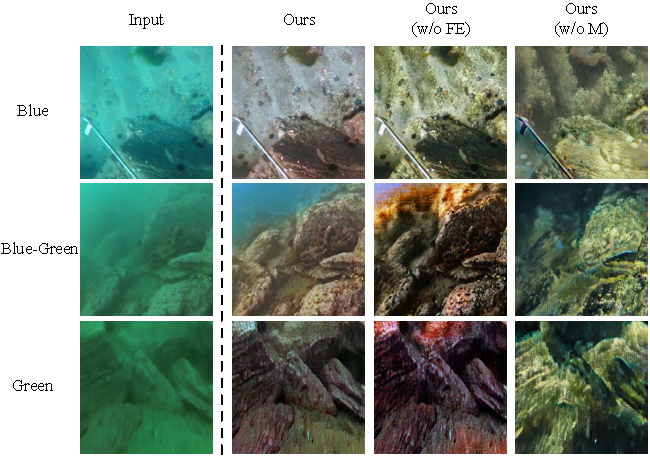
\includegraphics[width=\textwidth]{figs/RUIE_UCCS.pdf}
	\caption{我们的方法和去掉FE或M网络的方法在RUIE数据集的UCCS子集上的视觉效果。}
	\label{fig:RUIE_UCCS}
\end{figure*}

\begin{figure*}[!ht]
    \centering
	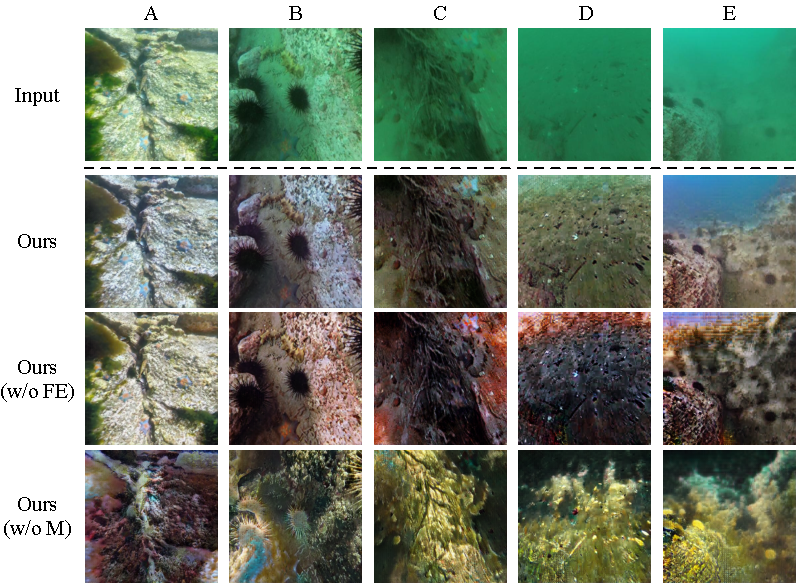
\includegraphics[width=\textwidth]{figs/RUIE_UIQS.pdf}
	\caption{我们的方法和去掉FE或M网络的方法在RUIE数据集的UIQS子集上的视觉效果。}
	\label{fig:RUIE_UIQS}
\end{figure*}

\subsubsection{映射网络的有效性验证实验}

图\ref{fig:RUIE_UCCS}和图\ref{fig:RUIE_UIQS}展示了在原有方法的基础上去掉映射网络(记作our (w/o M))的效果,如果说去掉特征提取网络使我们的网络局限于处理轻微浑浊的水下图像,那么去掉映射网络则直接导致我们的方法无法进行水下图像清晰化任务,因为从图中可以明显看出无论色调和浑浊度如何变化,去掉映射网络的方法都无法保证信息的完整性,进一步反映出在翻译前将水下信息特征与清晰图像信息空间对齐的重要性。

\section{讨论}

从前面的实验和分析中可以看出,尽管我们的方法与最先进的方法相比可以获得令人满意的结果,但仍存在几个问题:一是对于有浓雾且为开阔海域的水下图像,我们的方法不能生成很平滑的背景,推断可能是受数据集的影响,尽管训练使用的数据集是非配对的,但仍需要水下图像域和清晰图像域都包含各种场景,有浓雾且为开阔海域的水下图像容易拍摄,但这一类型的清晰图像难以获得,训练时,我们的方法在清晰域没有学习到这类图像的清晰化结果,从而影响翻译效果。二是在清晰度上仍有待加强,消融实验的结果显示去掉特征提取网络可以从浑浊程度较轻的水下图像翻译出清晰的图像,但它无法翻译浑浊水下图像,加入特征提取网络的方法则通过损失少量清晰度来实现浑浊水下图像的清晰化,后续我们会继续研究如何同时兼顾二者,以获得更清晰、适用范围更广泛的水下图像清晰化算法。

\section{本章小结}

本章将基于生成对抗网络的图像翻译应用到水下图像清晰化任务中,并针对此任务设计了我们的分解表示模型。

在第一节中,我们介绍了水下图像清晰化的意义和实用价值,以及基于生成对抗网络的方式解决清晰化问题的优势。

在第二节中,我们介绍了水下光学特性,指出水下成像受吸收和散射影响,导致水下图像存在低对比度、色偏、有雾状效果和噪声等问题。

在第三节中,我们依据水下光学特性提出我们的分解表示模型,将吸收和散射的影响分开考虑,并将分解得到的特征再映射以获得更清晰的效果。我们对再映射用到的特征提取网络和映射网络做细致描述,并介绍了所有的损失函数,最终我们给出了网络的总损失函数,实现了网络端到端的训练优化。

在第四节中,我们设计了水下图像清晰化实验,在4个数据集上证明了我们的方法的优势,并设计了消融实验,以验证特征提取网络和映射网络的有效性。

在最后一节中,我们讨论了我们的方法存在的局限性,为后续研究指明方向。




